\section{Deep learning}
\label{sec:deeplearning}
%
Deep learning lies at the heart of the most advanced machine learning solutions,
such as those that have learned to recognize items and images, determine the
sentiment of text, and drive vehicles. 
These neural networks are complex and can be challenging to build, but Keras 
removes much of the effort.
Keras acts as an API\footnote{An Application Programming Interface (API) 
provides an abstraction for a problem and specifies how clients should interact 
with the software componentes that implement a solution to that
problem.\cite{api}}, 
letting us quickly create a network that might take hours or days to hand code 
in Python or other languages.
%
\subsection{Introducing Keras}
\label{sec:introduction_keras}
Let's use the definition from the documentation at keras.io.
Keras is a high-level neural network API, written in Python and capable of
running on top of TensorFlow, CNTK or Theano.\cite{chollet2015keras}
That is, it lets us build neural networks easier by providing us with a
high-level set of constructs.
These constructs handle much of the plumbing involving in wring up neural
networks and thus reduce programming errors.
Also, as an API, it provides an interface that we can develop against and a
detailed description of what happens when we invoke various objects and methods.
Keras is Python centric in its code and is implemented as a Python library.
It is imported and used just like any other Python library you might be familiar
with, so the learning curve is minimal.
Finally, Keras runs on top of \emph{TensorFlow}, \emph{CNTK}, or \emph{Theano}.
These are three of the most widely used libraries for performing work with
neural networks.
Keras calls these libraries to perform the actual execution of operations that
create, populate, train, and evaluate the neural networks we specify in Keras.
Keras utilizes either TensorFlow, CNTK, or Theano as the 
\emph{backend}\footnote{In software engineering, the terms front end and back 
end refer to the separation of concerns between the presentation layer (front 
end), and the data access layer (back end) of a piece of software, or the 
physical infrastructure or hardware. In the client--server model, the client 
is usually considered the front end and the server is usually considered the 
back end, even when some presentation work is actually done on the server.
\cite{backend}}.
Keras itself does not create or execute the neural network.
Rather, Keras defines an API we code against. 
In our code we invoke Keras methods and pass the appropriate parameters.
Keras evaluates these for correctness and constructs whatever objects are
required.
Keras then calls the appropriate backend methods to do the actual neural 
network operations, such as defining structures, training the neural network 
model, and evaluating the trained model. Any result from these operations are 
returned by the backend to Keras, which processes them and returns to our code 
the appropriate results.
%
\begin{figure}[!h]
\centering
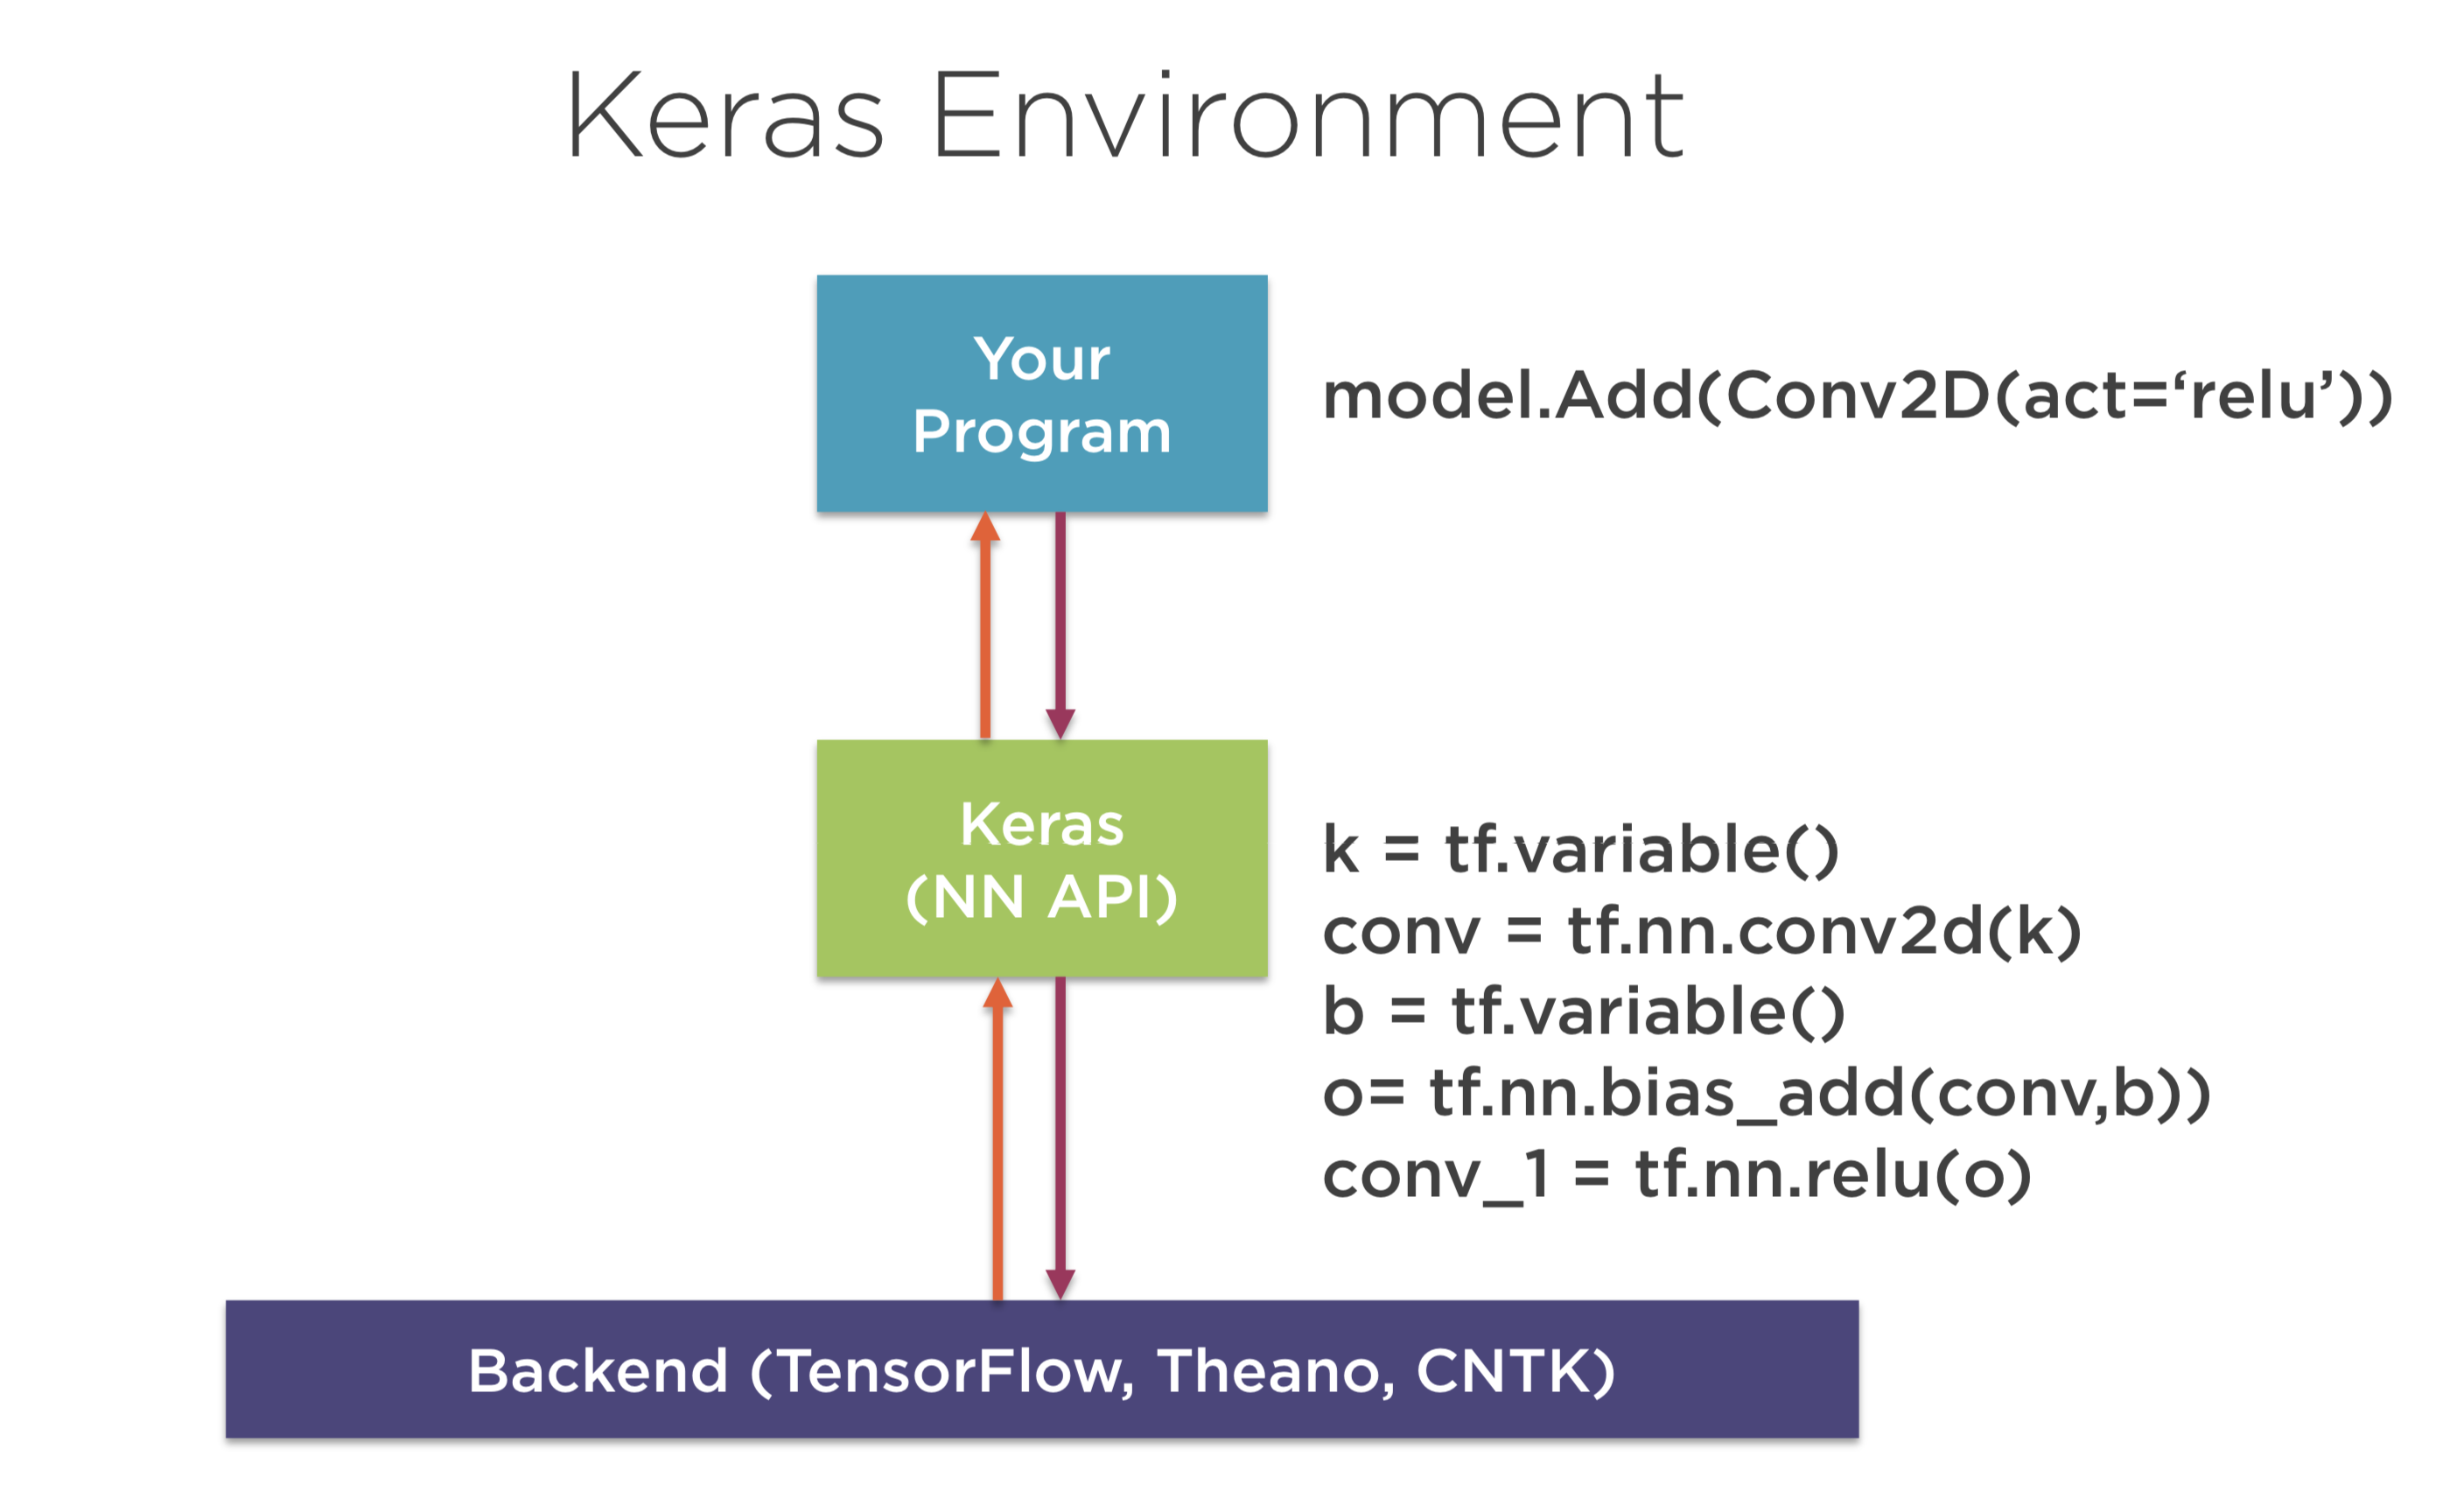
\includegraphics[width=\linewidth]{enviroment}
\caption{Keras enviroment}
\label{fig:nn_layer}
\end{figure}
%
\section{Neural Networks}
\label{sec:neuralnetwork}
%
The neural network, in figure \ref{fig:nn_layer}, where on the 
left we have the input layer, which feeds data into the network.
This data could be values from a data table, images from a camera, sounds from a
recording, or output from a sensor.
The input layer does not change the data, it simply passes it for processing by
the remaining layers. The data from the input layer is passed to another layer
of neurons.
These layers can be of different types with the different layer types performing
different transformations on the data as required by our solution. In a simple
network, the input layer can be directly connected to an output layer of neurons,
which provide the final outputs.
%
\begin{figure}[!h]
\centering
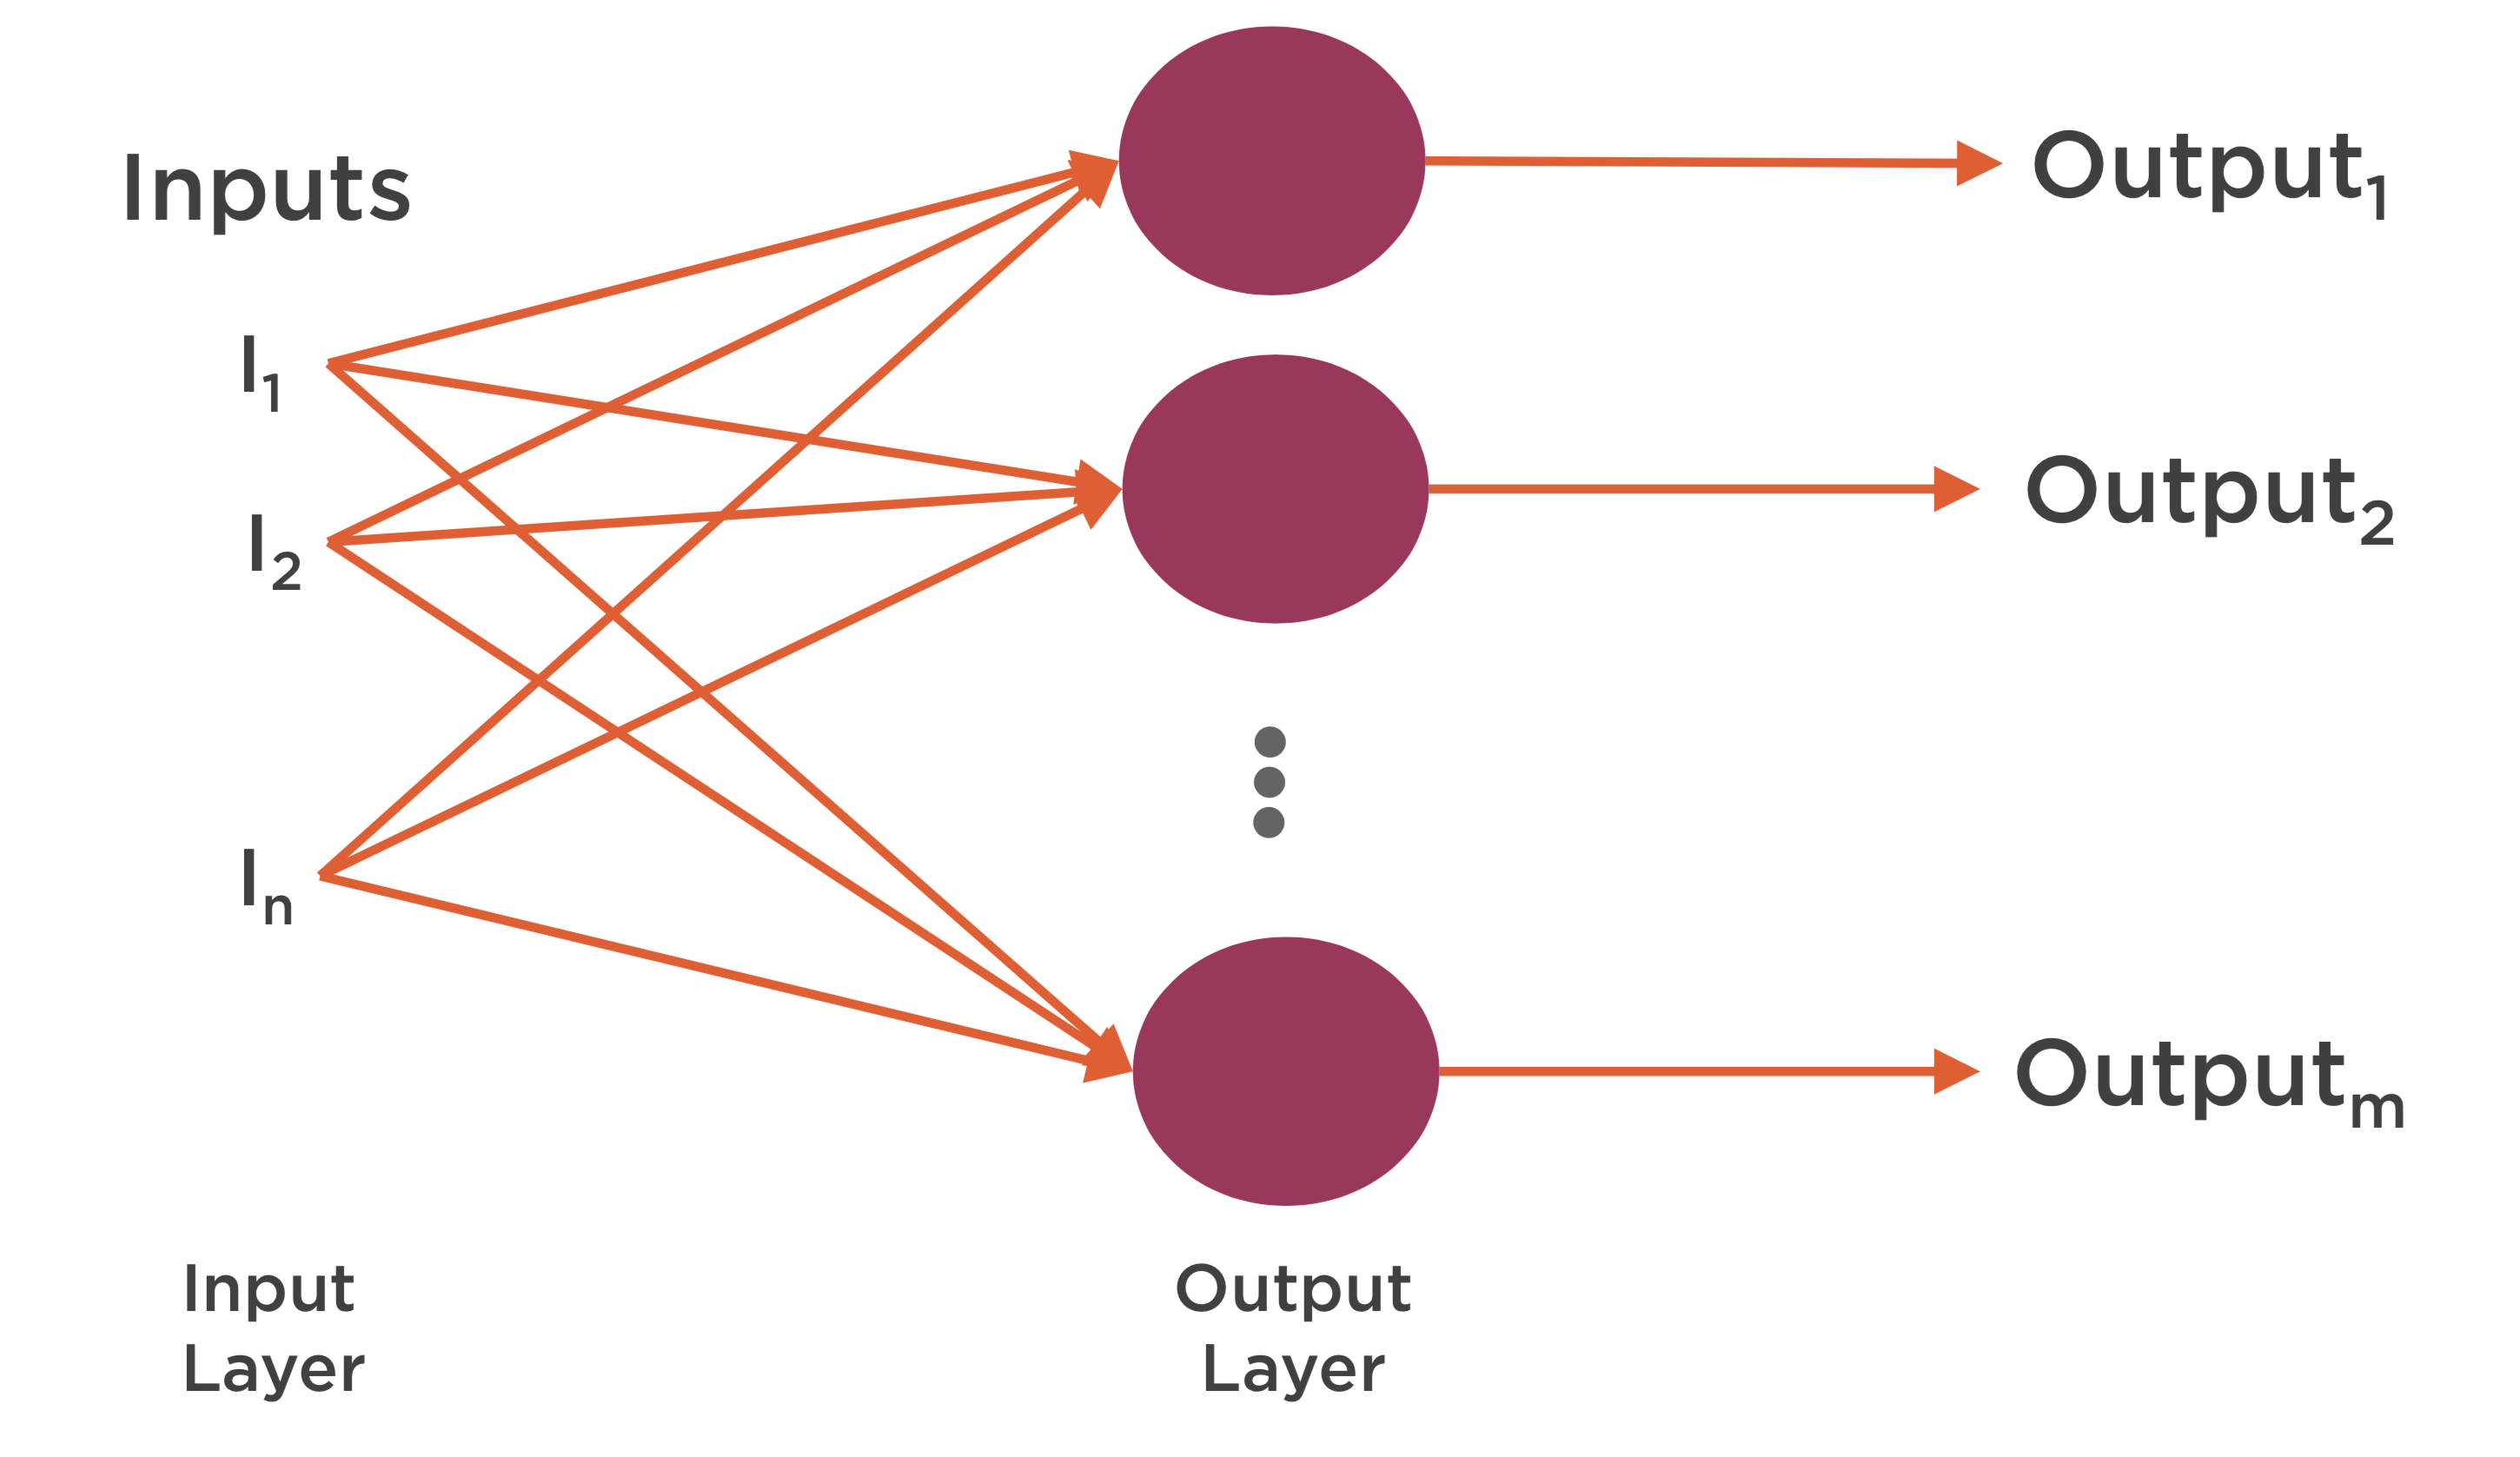
\includegraphics[width=\linewidth]{neuralnetwork}
\caption{Neural networks layers}
\label{fig:nn_layer}
\end{figure}
%
But in most networks, the input layer is connected to hidden layers.
Hidden layers are defined as not being input or output layers, and therefore,
are hidden to the code that's using the neural network.
The network can have many hidden layers and if there are two or more hidden
layers we call the network a deep neural network.
%
\begin{figure}[!h]
\centering
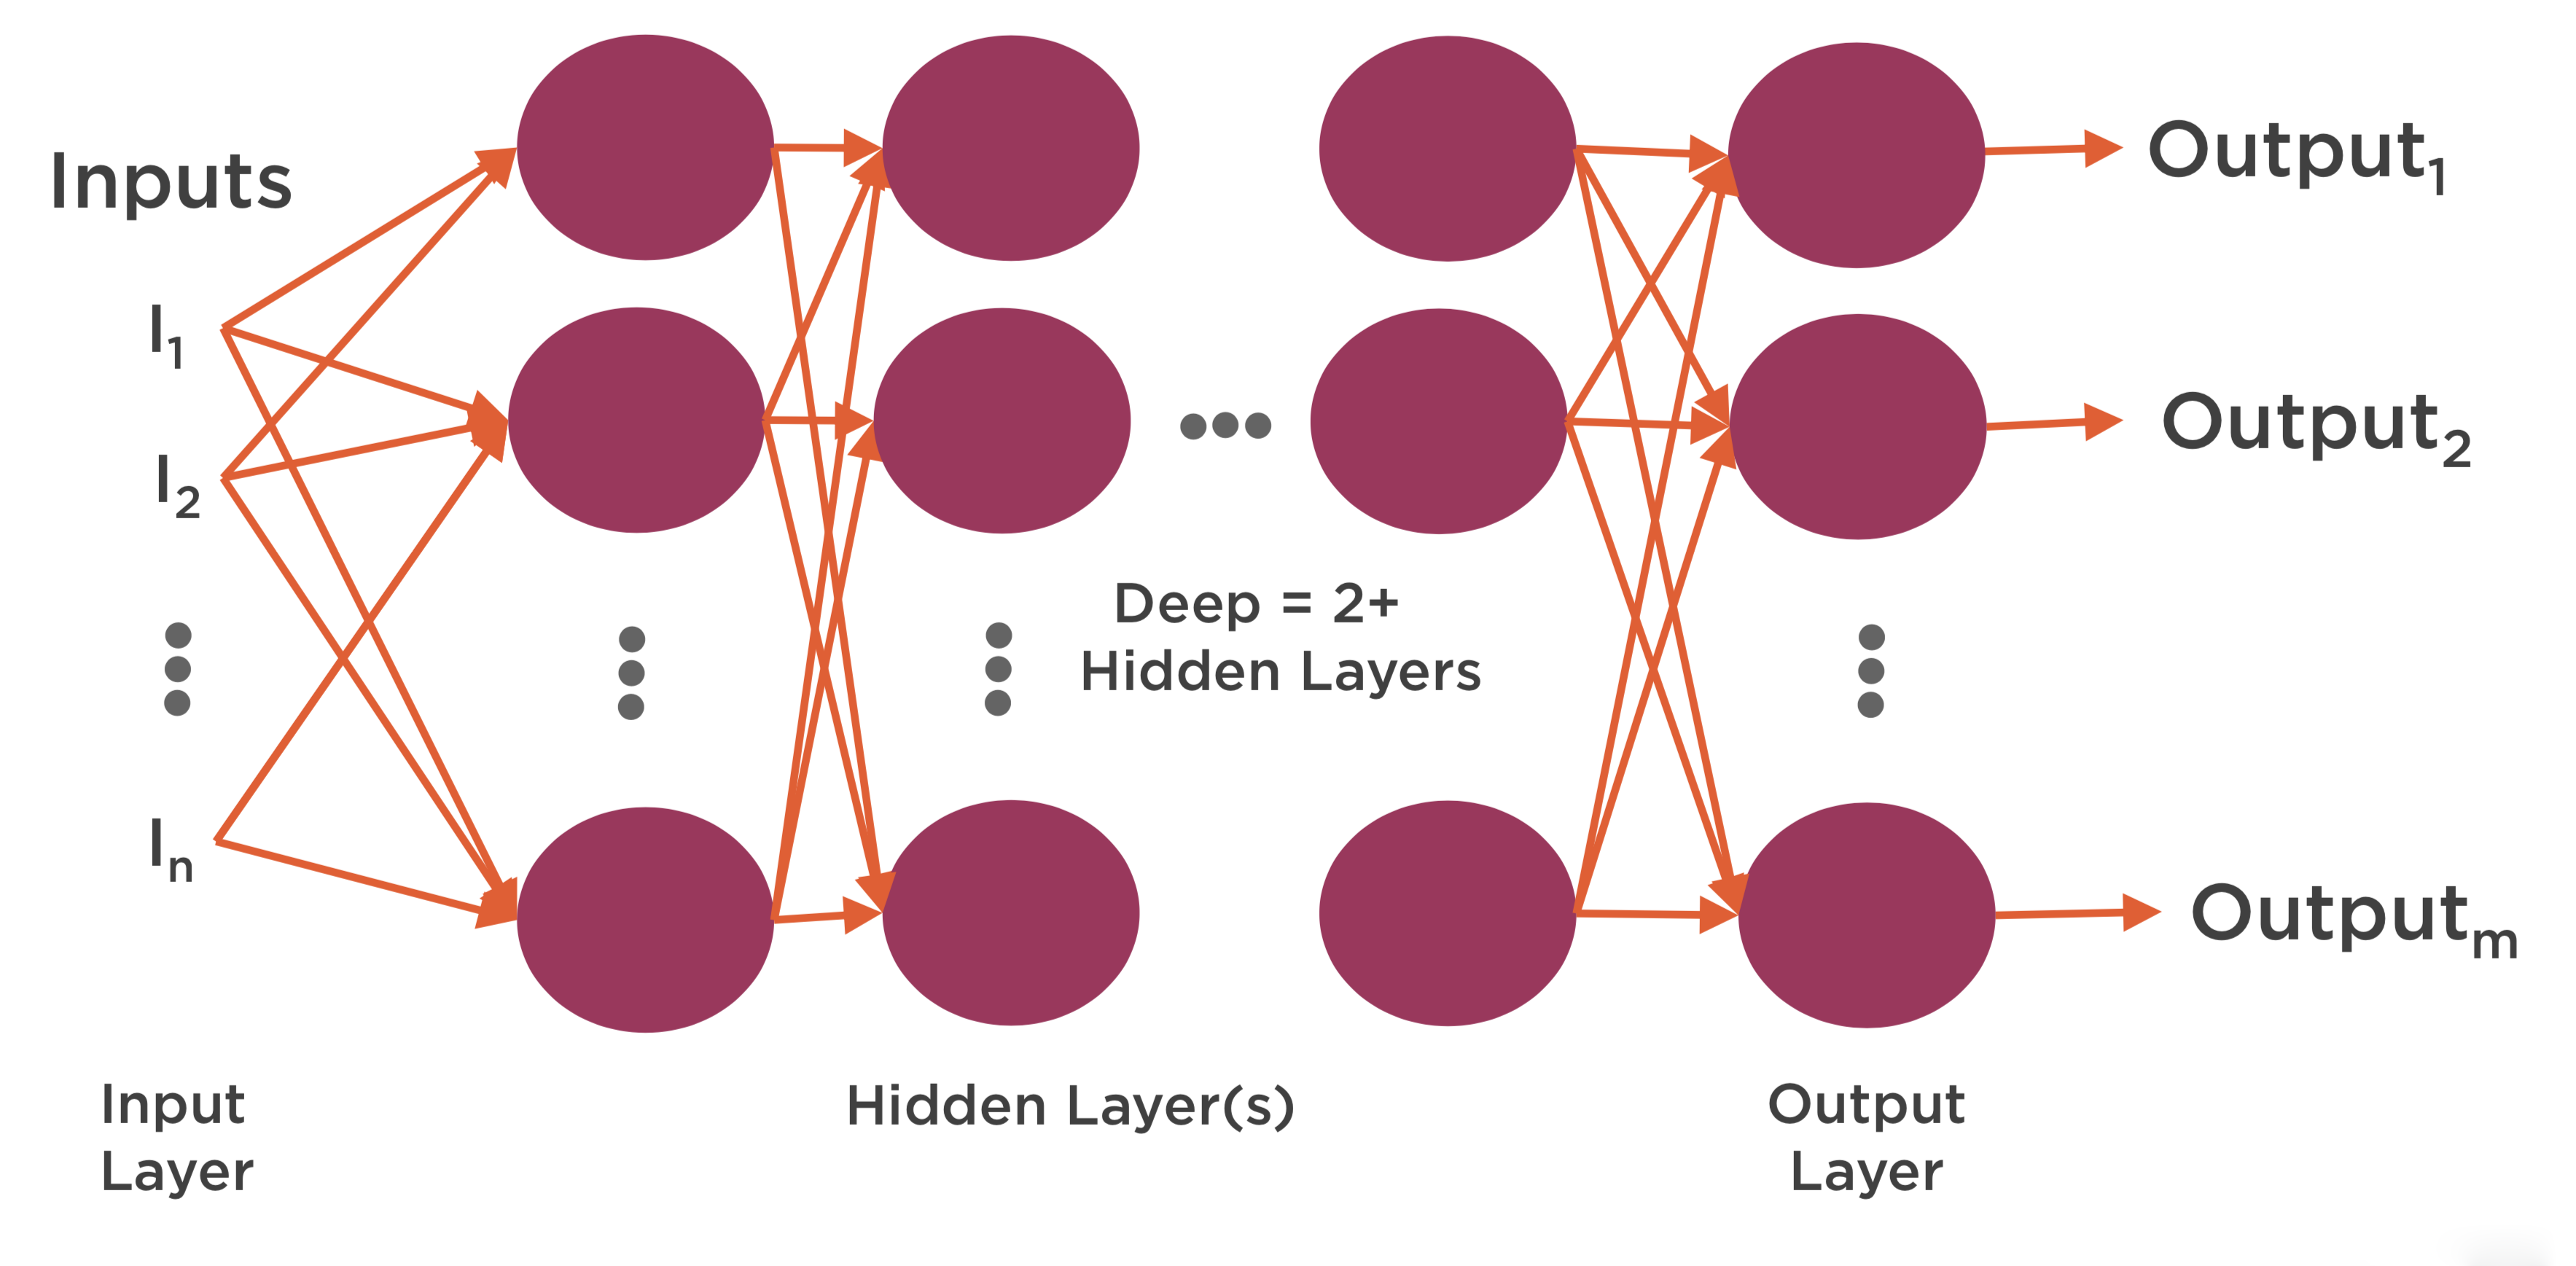
\includegraphics[width=\linewidth]{deep_nn}
\caption{Deep neural networks layers}
\label{fig:deepnn}
\end{figure}
%
In this learning process we adjust the structures of our neurons.
To understand this, let's look at a single neuron. Here we see the inputs and
outputs we showed in the network diagram, with the inputs going in and the
outputs going out.
However, what is not showing in this diagram is how the neurons work internally.
To do that, we need to open the neuron so we can see how it is constructed.
As we see, the neuron is performing a simple mathematics summing of weights times
the input value and adding a bias.
The product of these operations is passed through a non-linear activation function.
And the output of the activation function is the output of the neuron.
A key feature of the neural network is the ability to use the input data to
train the weights and biases so the signal passed out of the neuron changes
based on the input data. To do this training, we expose the network to data.
With each set of data, an algorithm is used to adjust the weights and bias to
minimize the error the network has in predicting the data's values.
This is done through processes called forward propagation and back propagation.
And when these processes are complete, the network is said to be trained, and
the weights and biases of all the neurons have been adjusted to give the best
results on the training data. So to summarize, the neural network consists of
three layer types, input, hidden, and output. 
By passing training data through the network, the network of neurons is 
trained to give results with the least error.
This training is done by adjusting weights and biases in the neurons, utilizing
the processes of forward propagation and back propagation, and if there are two
or more hidden layers in the network, we say it's a deep neural network.
